\section[ann]{Artificial Neural Networks / Deep Learning}


\begin{frame}
\frametitle{Applying Neural Networks: Forward Propagation}

  \def\layersep{2.5cm}
  \begin{center}
  \begin{tikzpicture}[shorten >=1pt,->,draw=black!50, node distance=\layersep]

    \draw[draw=none] (-3,2) rectangle (8,-4);
    \node[box=blue,opacity=.3,text opacity=1] at (0,1.5) {$\begin{array}{c}x = 2 \\ y = -1\end{array}$};
    \tikzstyle{every pin edge}=[<-,shorten <=1pt]
    \tikzstyle{neuron}=[circle,draw=black,fill=white,minimum size=17pt,inner sep=0pt]

    \draw<2-> node[neuron, fill=tree700, pin=left:x] (I-x) at (0,-1) {2};
    \draw<2-> node[neuron, fill=tree400, pin=left:y] (I-y) at (0,-2) {-1};
    \draw<1> node[neuron, fill=white, pin=left:x] (I-x) at (0,-1) {}; 
    \draw<1> node[neuron, fill=white, pin=left:y] (I-y) at (0,-2) {}; 
    
    \draw<5-> node[neuron, fill=tree800] (H-1) at (\layersep,-0.5) {0.8};
    \draw<5-> node[neuron, fill=tree700] (H-2) at (\layersep,-1.5) {0.5};
    \draw<5-> node[neuron, fill=tree300] (H-3) at (\layersep,-2.5) {-0.5};
    \draw<4> node[neuron, fill=tree800] (H-1) at (\layersep,-0.5) {2.5};
    \draw<4> node[neuron, fill=tree700] (H-2) at (\layersep,-1.5) {1.0};
    \draw<4> node[neuron, fill=tree300] (H-3) at (\layersep,-2.5) {-1};
    \draw<1-3> node[neuron, fill=white] (H-1) at (\layersep,-0.5) {}; 
    \draw<1-3> node[neuron, fill=white] (H-2) at (\layersep,-1.5) {}; 
    \draw<1-3> node[neuron, fill=white] (H-3) at (\layersep,-2.5) {}; 

    \draw<8> node[neuron,fill=tree900,pin={[pin edge={->}]right:$f(\vec{x})$}, right of=H-2] (O) {0.8};
    \draw<7> node[neuron,fill=tree900,pin={[pin edge={->}]right:$f(\vec{x})$}, right of=H-2] (O) {2.3};
    \draw<1-6> node[neuron,fill=white,pin={[pin edge={->}]right:$f(\vec{x})$}, right of=H-2] (O) {}; 
    
    \draw<1-2>[line width=1pt, color=black] (I-x) -> (H-1);
    \draw<1-2>[line width=0.5pt, color=black] (I-x) -> (H-2);
    \draw<1-2>[line width=0.8pt, color=black] (I-x) -> (H-3);
    \draw<1-2>[line width=0.6pt, color=black] (I-y) -> (H-1);
    \draw<1-2>[line width=0.8pt, color=black] (I-y) -> (H-2);
    \draw<1-2>[line width=0.3pt, color=black] (I-y) -> (H-3);
    
    \draw<3->[line width=1pt, color=tree1000] (I-x) -> (H-1) node[pos=0.7,above=-0.1,sloped] {\tiny $2 \cdot 1.0$};
    \draw<3->[line width=0.5pt, color=tree700] (I-x) -> (H-2) node[pos=0.7,above=-0.1,sloped] {\tiny $2 \cdot 0.8$};
    \draw<3->[line width=0.8pt, color=tree200] (I-x) -> (H-3) node[pos=0.7,above=-0.1,sloped] {\tiny $2 \cdot -0.8$};
    \draw<3->[line width=0.6pt, color=tree300] (I-y) -> (H-1) node[pos=0.3,above=-0.1,sloped] {\tiny ${-1} \cdot {-0.5}$};
    \draw<3->[line width=0.8pt, color=tree800] (I-y) -> (H-2) node[pos=0.3,above=-0.1,sloped] {\tiny ${-1} \cdot 0.6$};
    \draw<3->[line width=0.8pt, color=tree200] (I-y) -> (H-3) node[pos=0.3,above=-0.1,sloped] {\tiny ${-1} \cdot {-0.6}$};
            
    \draw<1-5>[line width=0.7pt, color=black] (H-1) -> (O);
    \draw<1-5>[line width=1.3pt, color=black] (H-2) -> (O);
    \draw<1-5>[line width=1.1pt, color=black] (H-3) -> (O);
        
    \draw<6->[line width=0.7pt, color=tree700] (H-1) -> (O) node[pos=0.5,above=-0.1,sloped] {\tiny $0.8 \cdot 0.5$};
    \draw<6->[line width=1.3pt, color=tree900] (H-2) -> (O) node[pos=0.5,above=-0.1,sloped] {\tiny $0.5 \cdot 3.0$};
    \draw<6->[line width=1.1pt, color=tree300] (H-3) -> (O) node[pos=0.5,above=-0.1,sloped] {\tiny ${-0.5} \cdot {-0.8}$};

    \draw node[above of=H-1, node distance=1cm] (hl) {Hidden layer};
    \draw node[left of=hl] {Input layer};
    \draw node[right of=hl] {Output layer};

    \draw<2> node[below of=H-3, node distance=1cm] (desc) {Assign features to input neurons};
    \draw<3> node[below of=H-3, node distance=1cm] (desc) {Multiple input neuron activation $x_i$ with their weights $w_{ij}$};
    \draw<4> node[below of=H-3, node distance=1cm] (desc) {Hidden neurons sum up their inputs $a_h = \sum_i x_i w_{ih}$};
    \draw<5> node[below of=H-3, node distance=1cm] (desc) {Hidden neurons apply their activation function $x_h = \sigma(a_h)$};
    \draw<6> node[below of=H-3, node distance=1cm] (desc) {Multiple hidden neuron activation $x_h$ with their weights $w_{ho}$};
    \draw<7> node[below of=H-3, node distance=1cm] (desc) {Output neuron sums up its inputs $a_o = \sum_h x_h w_{ho}$};
    \draw<8> node[below of=H-3, node distance=1cm] (desc) {Output neuron applies its activation function $x_o = \sigma(a_o)$};
\end{tikzpicture} 
\end{center}
\end{frame}


\begin{frame}
\frametitle{Training Neural Networks: Backpropagation}

  \def\layersep{2.5cm}
  \begin{tikzpicture}[shorten >=1pt,->,draw=black!50, node distance=\layersep]

    \draw[draw=none] (-3,2) rectangle (7,-4);
    \node[box=blue,opacity=.3,text opacity=1] at (0,1.5) {$\begin{array}{c}x_o = 0.8 \\ t = 1\end{array}$};
    \tikzstyle{every pin edge}=[<-,shorten <=1pt]
    \tikzstyle{neuron}=[circle,draw=black,fill=white,minimum size=17pt,inner sep=0pt]

    \draw node[neuron, fill=white, pin=left:x] (I-x) at (0,-1) {};
    \draw node[neuron, fill=white, pin=left:y] (I-y) at (0,-2) {};
            
    \draw<5-> node[neuron, fill=tree800] (H-1) at (\layersep,-0.5) {0.1};
    \draw<5-> node[neuron, fill=tree700] (H-2) at (\layersep,-1.5) {0.2};
    \draw<5-> node[neuron, fill=tree300] (H-3) at (\layersep,-2.5) {-0.3};
    \draw<1-4> node[neuron, fill=white] (H-1) at (\layersep,-0.5) {};
    \draw<1-4> node[neuron, fill=white] (H-2) at (\layersep,-1.5) {};
    \draw<1-4> node[neuron, fill=white] (H-3) at (\layersep,-2.5) {};

    \draw<2-> node[neuron,fill=tree900,pin={[pin edge={->}]right:$f(\vec{x})$}, right of=H-2] (O) {0.4};
    \draw<1> node[neuron,fill=white,pin={[pin edge={->}]right:$f(\vec{x})$}, right of=H-2] (O) {};
            
    \draw<1-6>[line width=1pt, color=black] (I-x) -> (H-1);
    \draw<1-6>[line width=0.5pt, color=black] (I-x) -> (H-2);
    \draw<1-6>[line width=0.8pt, color=black] (I-x) -> (H-3);
    \draw<1-6>[line width=0.6pt, color=black] (I-y) -> (H-1);
    \draw<1-6>[line width=0.8pt, color=black] (I-y) -> (H-2);
    \draw<1-6>[line width=0.3pt, color=black] (I-y) -> (H-3);
    
    \draw<7->[line width=1pt, color=tree1000] (I-x) -> (H-1) node[pos=0.7,above=-0.1,sloped] {\tiny $+0.4$};
    \draw<7->[line width=0.5pt, color=tree700] (I-x) -> (H-2) node[pos=0.7,above=-0.1,sloped] {\tiny $+0.3$};
    \draw<7->[line width=0.8pt, color=tree200] (I-x) -> (H-3) node[pos=0.7,above=-0.1,sloped] {\tiny $-0.2$};
    \draw<7->[line width=0.6pt, color=tree300] (I-y) -> (H-1) node[pos=0.3,above=-0.1,sloped] {\tiny $-0.2$};
    \draw<7->[line width=0.8pt, color=tree800] (I-y) -> (H-2) node[pos=0.3,above=-0.1,sloped] {\tiny $+0.3$};
    \draw<7->[line width=0.8pt, color=tree200] (I-y) -> (H-3) node[pos=0.3,above=-0.1,sloped] {\tiny $-0.4$};
        
    \draw<1-3>[line width=0.7pt, color=black] (H-1) -> (O);
    \draw<1-3>[line width=1.3pt, color=black] (H-2) -> (O);
    \draw<1-3>[line width=1.1pt, color=black] (H-3) -> (O);
    
    \draw<4->[line width=0.7pt, color=tree700] (H-1) -> (O) node[pos=0.5,above=-0.1,sloped] {\tiny $+0.2$};
    \draw<4->[line width=1.3pt, color=tree900] (H-2) -> (O) node[pos=0.5,above=-0.1,sloped] {\tiny $+0.1$};
    \draw<4->[line width=1.1pt, color=tree300] (H-3) -> (O) node[pos=0.5,above=-0.1,sloped] {\tiny $+0.2$};

    \draw node[above of=H-1, node distance=1cm] (hl) {Hidden layer};
    \draw node[left of=hl] {Input layer};
    \draw node[right of=hl] {Output layer};
    
    \draw<1> node[below of=H-3, node distance=2cm, text width=\textwidth] (desc) {Adapt weights using gradient descent on loss function
    \begin{align*}
      \Delta w &= - \eta \frac{\partial \mathcal{L}}{\partial w}
    \end{align*}
      };

    \draw<2> node[below of=H-3, node distance=2cm, text width=\textwidth] (desc) {Gradient of loss function with respect to the output
    \begin{align*}
      \mathcal{L} &= (x_o - t)^2  &  \frac{\partial \mathcal{L}}{\partial x_o} &= 2 (x_o - t)
    \end{align*}
      };

    \draw<3> node[below of=H-3, node distance=2cm, text width=\textwidth] (desc) {Gradient of output neuron with respect to the hidden weights
    \begin{align*}
      x_o &= \sigma(\sum_h x_h w_{ho}) & \frac{\partial x_o}{\partial w_{ho}} &= \sigma'(\sum_h x_h w_{ho}) x_h
    \end{align*}
      };
    
    \draw<4> node[below of=H-3, node distance=2cm, text width=\textwidth] (desc) {Adapt hidden weights
    \begin{align*}
      \Delta w_{ho} &= - \eta  \frac{\partial \mathcal{L}}{\partial x_o} \frac{\partial x_o}{\partial w_{ho}}
    \end{align*}
      };
    
    \draw<5> node[below of=H-3, node distance=2cm, text width=\textwidth] (desc) {Gradient of loss function with respect to the hidden output
    \begin{align*}
      \frac{\partial \mathcal{L}}{\partial x_h} &=  \frac{\partial \mathcal{L}}{\partial x_o} \frac{\partial x_o}{\partial x_h} &  \frac{\partial x_o}{\partial x_h} &=   \sigma'(\sum_h x_h w_{ho}) w_{ho}
    \end{align*}
      };
    
    \draw<6> node[below of=H-3, node distance=2cm, text width=\textwidth] (desc) {Gradient of the hidden neurons with respect to the input weights
    \begin{align*}
      x_h &= \sigma(\sum_i x_i w_{ih}) &   \frac{\partial x_h}{\partial w_{ih}} &= \sigma'(\sum_i x_i w_{ih}) x_i
    \end{align*}
      };
    
    \draw<7> node[below of=H-3, node distance=2cm, text width=\textwidth] (desc) {Adapt the input weights
    \begin{align*}
      \Delta w_{ih} = - \eta  \frac{\partial \mathcal{L}}{\partial x_h} \frac{\partial x_h}{\partial w_{ih}}
    \end{align*}
      };
    
\end{tikzpicture} 

\end{frame}

\begin{frame}
    \frametitle{Summary: Feed-Forward Network}
    \begin{center}
      \begin{itemize}
        \item The data flows from the input to the output layer (feed-forward) 
            $$f(\vec{x}) = \sigma \left(\sum w^{\textrm{hid}}_{j} \sigma \left( \sum w^{\textrm{inp}}_i x_i \right) \right)$$
        \item Neurons sum up inputs and apply activation function $\sigma = $ 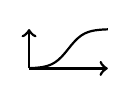
\begin{tikzpicture} 
            \draw[->,line width=1pt,Black] (0,0) -> (0,0.5);
            \draw[->,line width=1pt,Black] (0,0) -> (1,0);
            \draw[black, thick, domain=-5:5] plot ({\x/10 + 0.5}, {0.5/(1+exp(-\x))});
        \end{tikzpicture}
        \item The gradient of the loss-function flows from the output to the input layer and modifies the weights (back-propagation)
            $$\quad \quad \quad \quad \Delta w_{ij} = - \eta \frac{\partial L}{\partial w_{ij}} \quad \quad L = \left( f(\vec{x}) - t \right)^2$$
      \end{itemize}
      \vspace{-2em}


      \begin{tikzpicture}
          \node[anchor=south west,inner sep=0] (image) at (0,0) {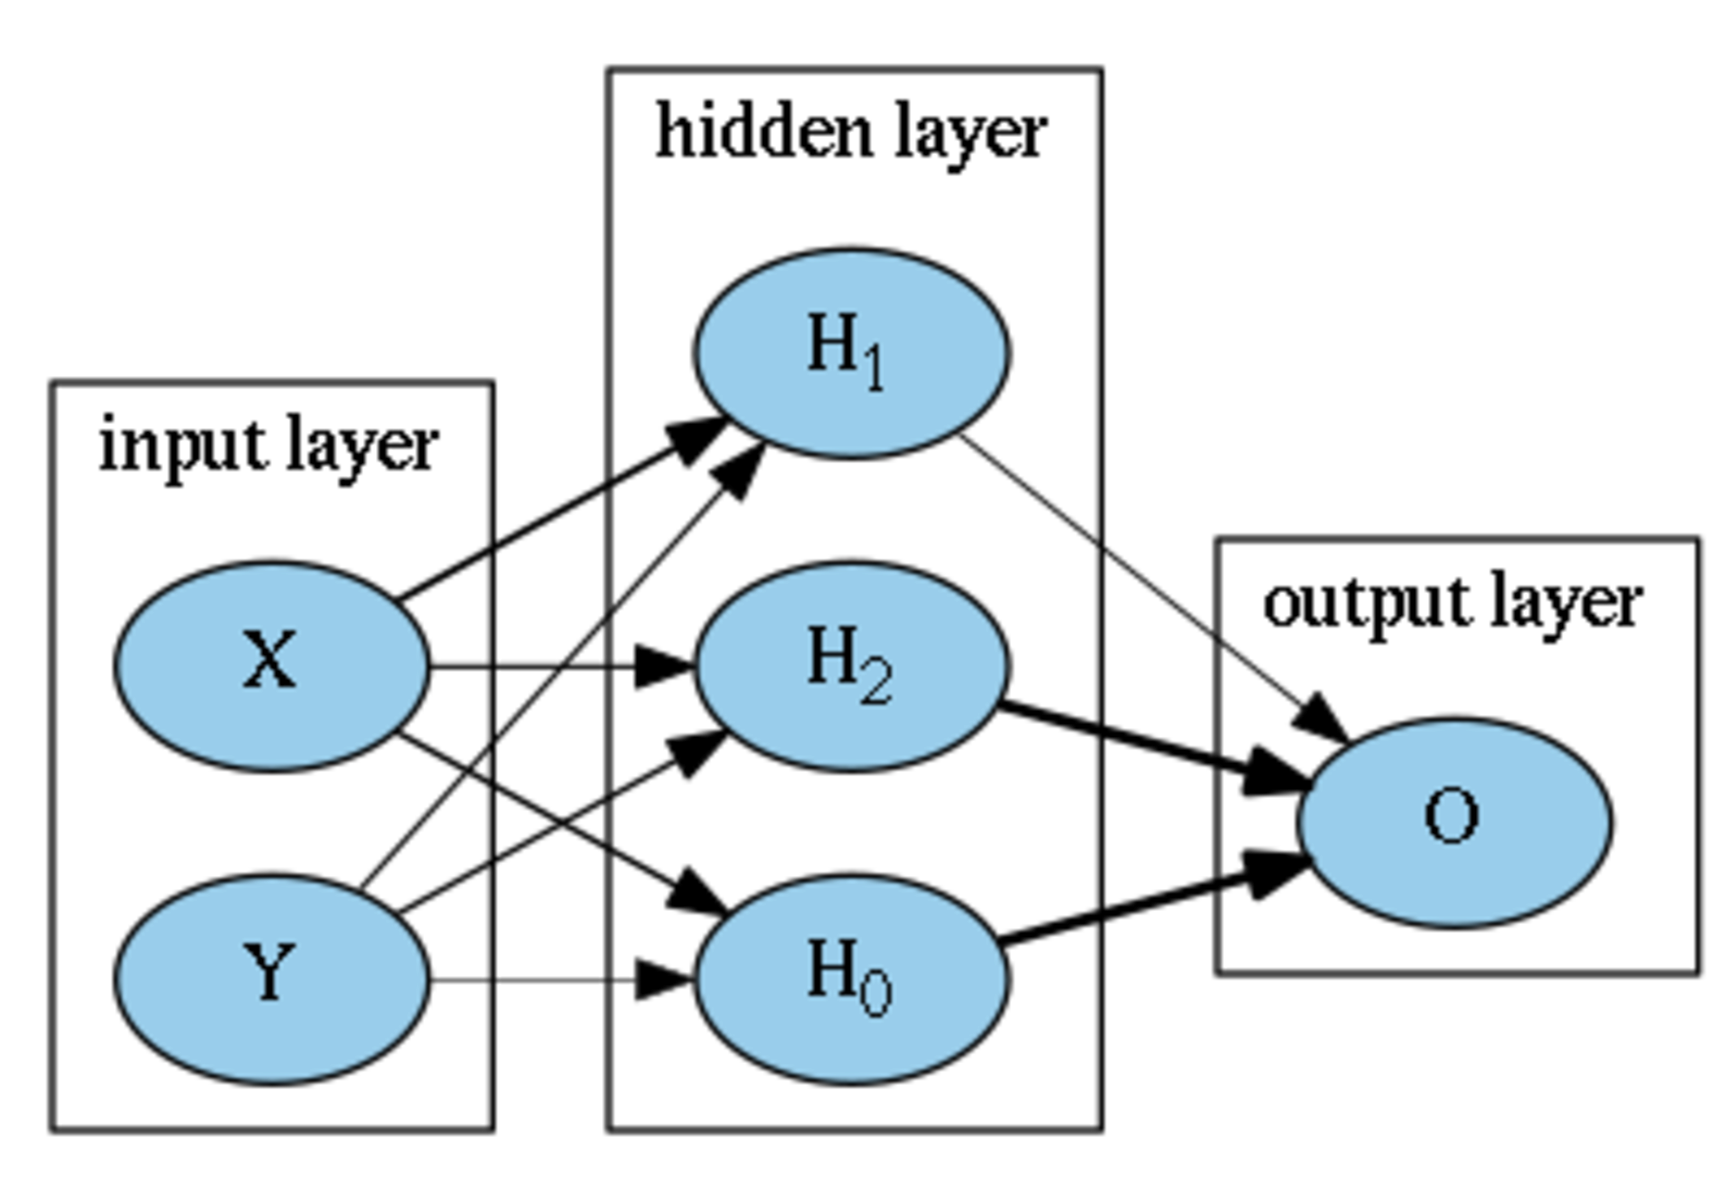
\includegraphics[width=0.5\textwidth]{mlp_visualization.png}};
          \node[anchor=south west,inner sep=0] (image) at (6,0) {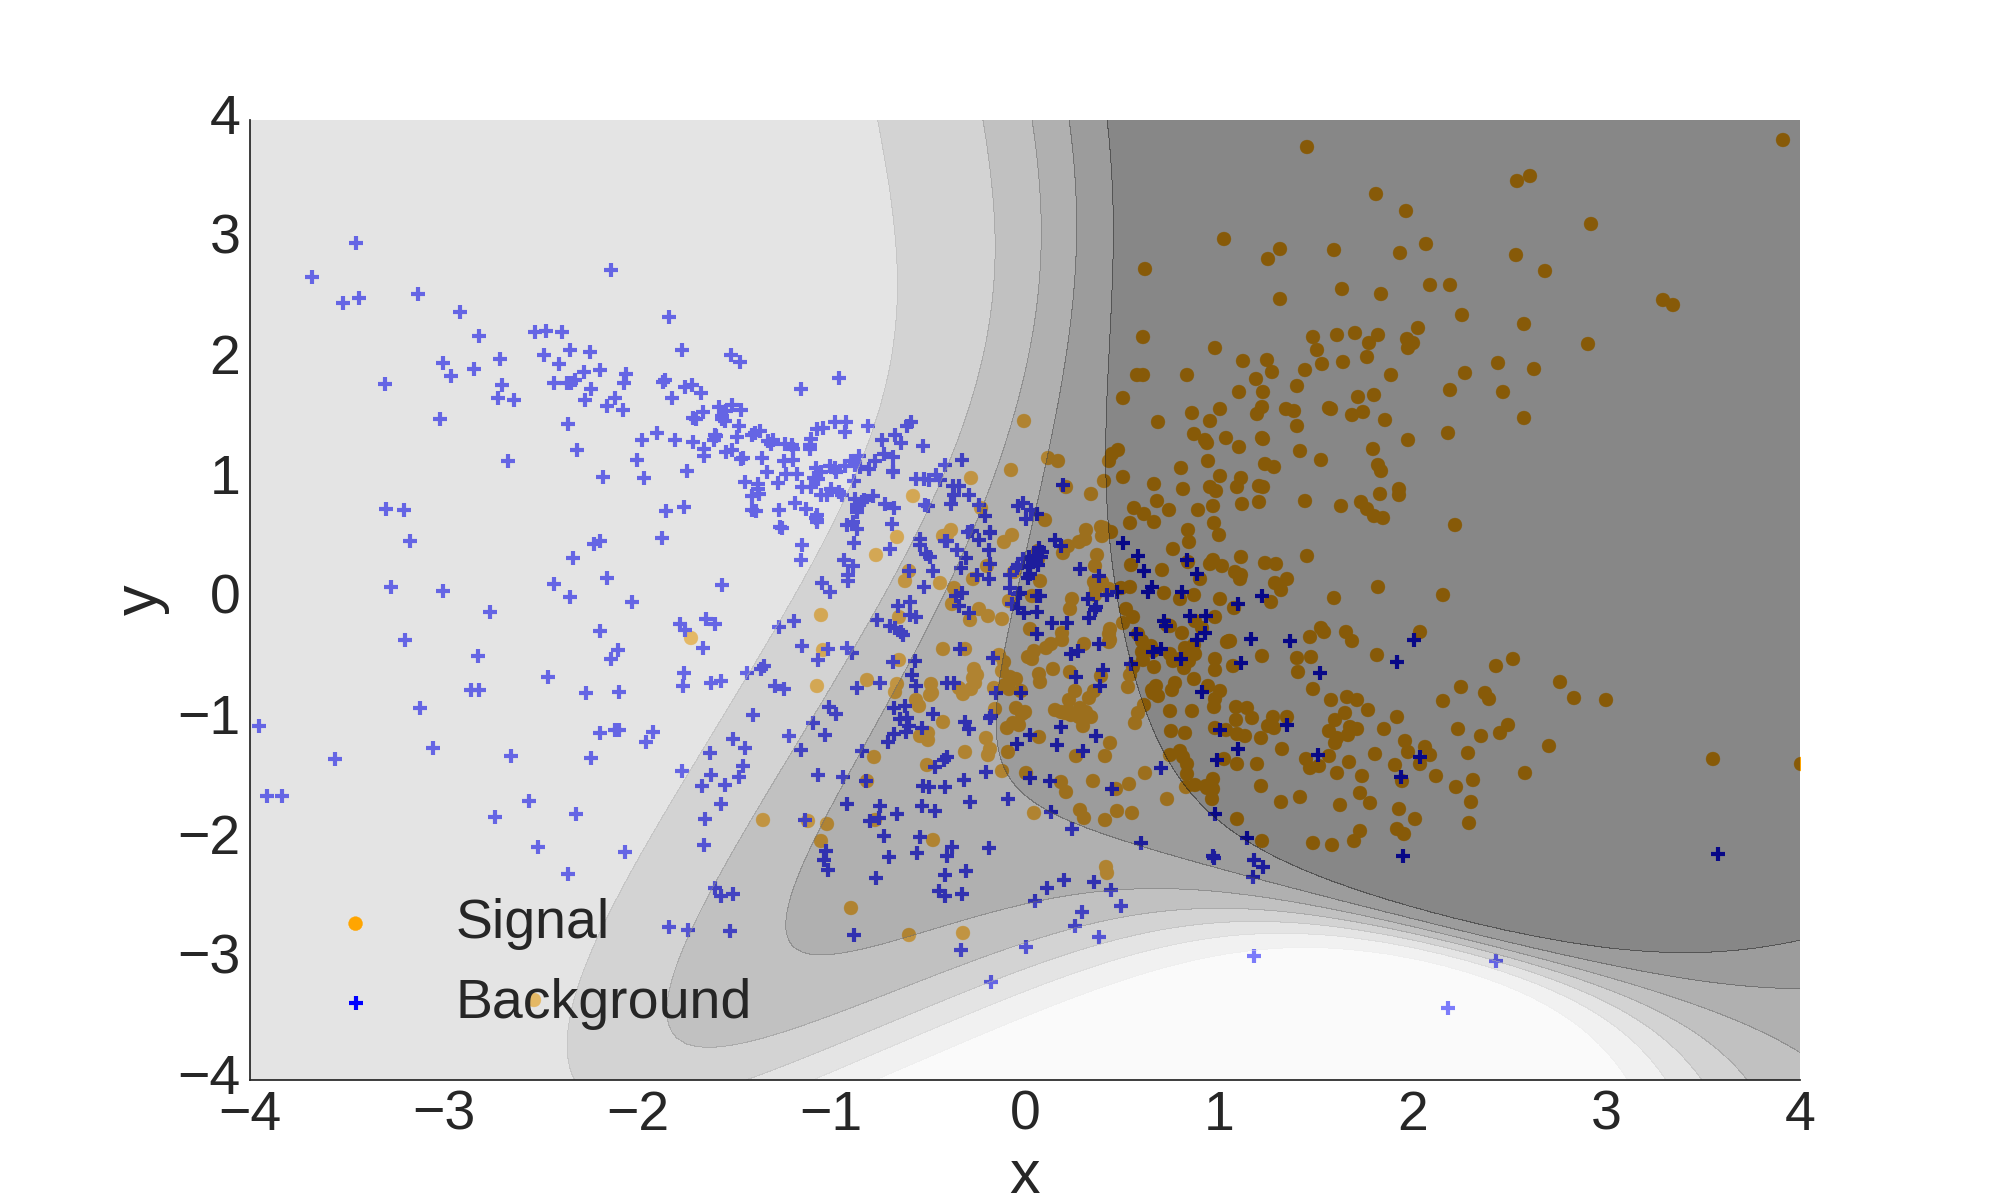
\includegraphics[width=0.5\textwidth]{mlp_classifier.png}};
      \end{tikzpicture}
    \end{center}
\end{frame}

\begin{frame}
    \frametitle{Common Activation Functions}
    \begin{center}
    
    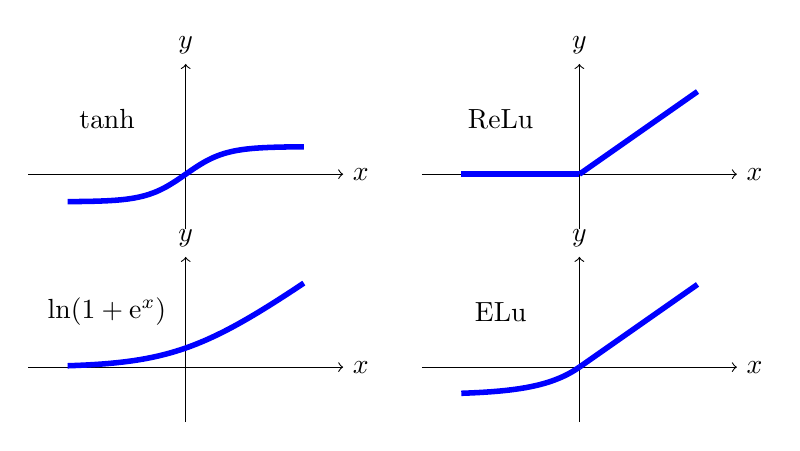
\begin{tikzpicture}[yscale=0.7]
		  \node at(-1,1) {$\tanh$};
          \draw[->] (-2,0) -- (2.0,0) node[right] {$x$};
          \draw[->] (0,-1) -- (0,2.0) node[above] {$y$};
          \draw[scale=0.5,domain=-3:3,smooth,variable=\x,blue,line width=2pt] plot ({\x},{tanh(\x)});
          
 		  \node at(-1,1-3.5) {$\ln(1+ \mathrm{e}^x)$};
          \draw[->] (-2,-3.5) -- (2.0,-3.5) node[right] {$x$};
          \draw[->] (0,-1-3.5) -- (0,2.0-3.5) node[above] {$y$};
          \draw[scale=0.5,domain=-3:3,smooth,variable=\x,blue,line width=2pt] plot ({\x},{ln(1+exp(\x)) - 7});
          
		  \node at(-1+5,1) {$\mathrm{ReLu}$};
          \draw[->] (-2+5,0) -- (2.0+5,0) node[right] {$x$};
          \draw[->] (0+5,-1) -- (0+5,2.0) node[above] {$y$};
          \draw[scale=0.5,domain=7:10,smooth,variable=\x,blue,line width=2pt] plot ({\x},{0});
          \draw[scale=0.5,domain=10:13,smooth,variable=\x,blue,line width=2pt] plot ({\x},{\x-10});
          
  		  \node at(-1+5,1-3.5) {$\mathrm{ELu}$};
            \draw[->] (-2+5,-3.5) -- (2.0+5,-3.5) node[right] {$x$};
            \draw[->] (0+5,-4.5) -- (0+5,-1.5) node[above] {$y$};
            \draw[scale=0.5,domain=7:10,smooth,variable=\x,blue,line width=2pt] plot ({\x},{exp(\x-10)-8});
            \draw[scale=0.5,domain=10:13,smooth,variable=\x,blue,line width=2pt] plot ({\x},{\x-17});

    \end{tikzpicture}
    
    \vspace{1em}
    \textbf{Desirable properties:} Nonlinear, Differentiable, Monotonic, Smooth
    \end{center}
\end{frame}

\begin{frame}
    \frametitle{Common Loss Functions}
    \begin{center}
    
    \begin{align*}
    \mathrm{Square} & &  \mathcal{L}(f(\vec{x}), y) &= \left(f(\vec{x}) - y\right)^2 \\
    \mathrm{Logistic Loss} & & \mathcal{L}(f(\vec{x}), y) &= \ln \left(1 + \mathrm{e}^{-y f(\vec{x})} \right) \\
    \mathrm{Cross Entropy} & &  \mathcal{L}(f(\vec{x}), t) &= -t \ln \left(f(\vec{x}) \right) - (1-t) \ln \left( 1 - f(\vec{x}) \right)
    \end{align*}
    
    \textbf{Loss Functions for neural networks must be differentiable}
    
     \end{center}
        
    \vspace{2em}
    \begin{small}
       \begin{align*}
       y &\in \left\lbrace -1, 1\right\rbrace \\
       t &\in \left\lbrace 0, 1 \right\rbrace
       \end{align*} 
    \end{small}
\end{frame}

\begin{frame}
    \frametitle{Selected aspects of training}
    \begin{center}
      \textbf{ANN yields small and fast models, but training can be challenging}
      \begin{align*}
        \Delta w_{ij} &= - \eta \frac{\partial L}{\partial w_{ij}}
      \end{align*}

      \begin{columns}
        \column{0.5\textwidth}
        \begin{itemize}
          \item Stochastic gradient-descent algorithm (Backpropagation)
            \begin{itemize}
              \item Batch-size
              \item Learning rate
              \item Momentum term (Adam)
              \item Hesse Matrix (BFGS)
            \end{itemize}
          \item Regularization
            \begin{itemize}
              \item Weight decay $\alpha \vec{w}^T \vec{w}$
              \item Dropout (ensemble)
            \end{itemize}
        \end{itemize}
        \column{0.5\textwidth}
        \begin{itemize}
          \item Architecture
            \begin{itemize}
              \item Number of neurons
              \item Number of layers
              \item Activation function
            \end{itemize}
          \item Initalization
            \begin{itemize}
              \item Usually gaussian distributed
              \item Xavier initialization $\mathrm{Var}(w_{ij}) = \frac{1}{N}$
            \end{itemize}
        \end{itemize}
      \end{columns}
    \end{center}
\end{frame}

\begin{frame}
    \frametitle{Example Classifier Quality}
    \begin{center}
      \begin{tikzpicture}
          \node[anchor=south west,inner sep=0] (image) at (0,0) {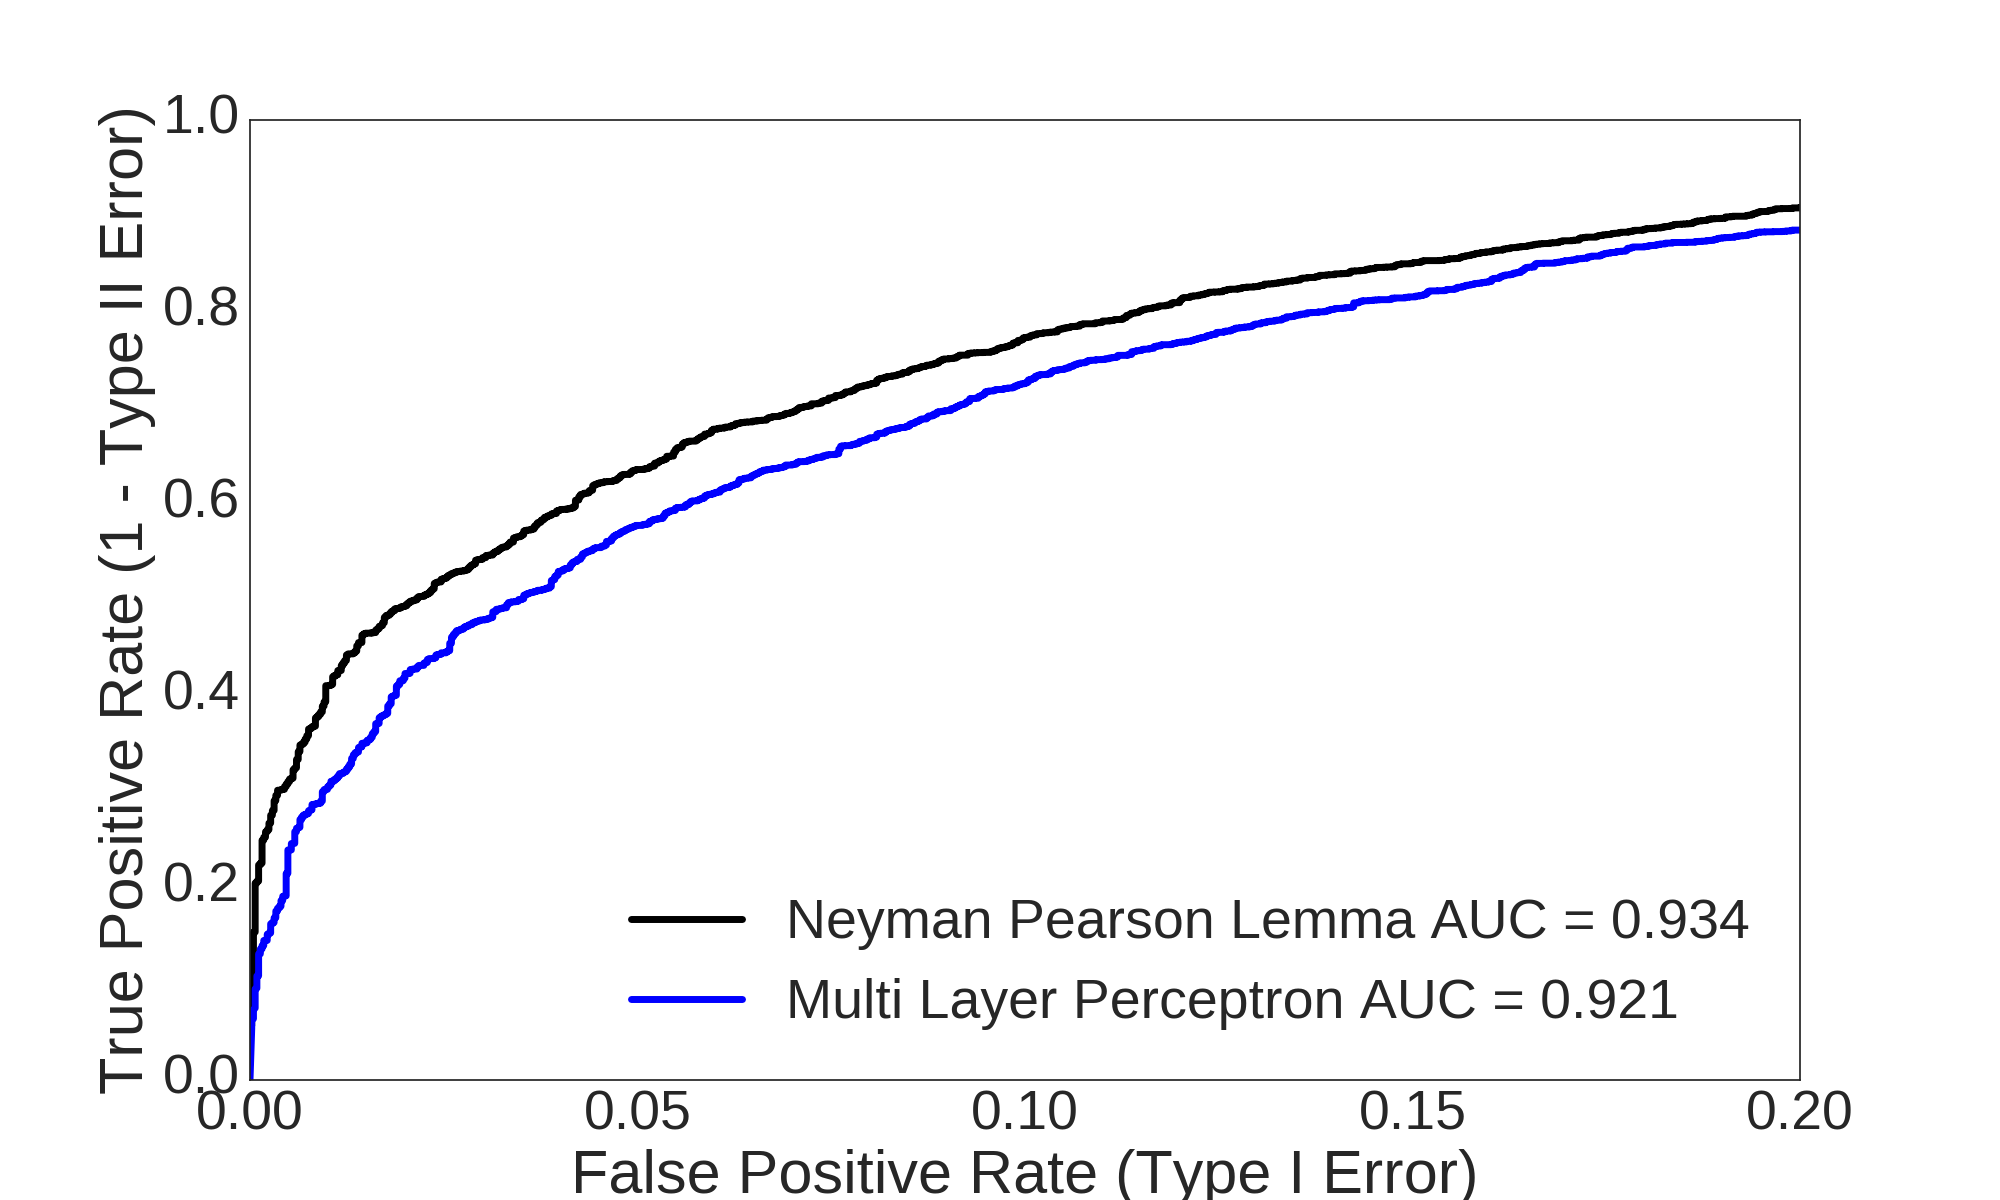
\includegraphics[width=\textwidth]{mlp_roc.png}};
      \end{tikzpicture}
    \end{center}
\end{frame}


\begin{frame}
    \frametitle{History (stay with me it's fun!)}
    \begin{center}
      \begin{itemize}
        \item Field started in the 1950s
        \item ... and died 1969 (Minsky and Papert)
        \item Assumed incapability to perform operations like exclusive-or
        \item Lack of computing power
      \end{itemize}
      

      \vspace{1em}
      \textbf{Perceptron}


      \begin{tikzpicture}
        \node[anchor=south west,inner sep=0] (image) at (0,0) {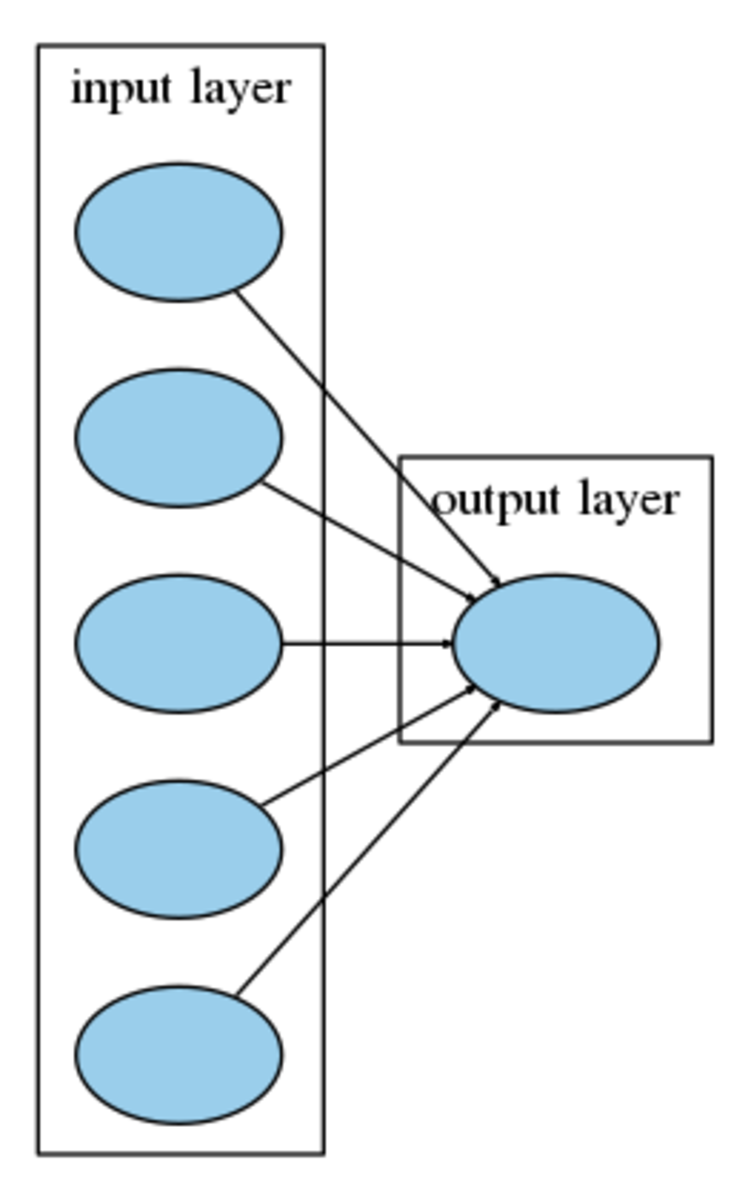
\includegraphics[height=0.3\textwidth]{ann_1_visualization.png}};
      \end{tikzpicture}
    \end{center}
\end{frame}

\begin{frame}
    \frametitle{History (stay with me it's fun!)}
    \begin{center}
      \begin{itemize}
        \item Field revolutionized in the 1980s by backpropagation algorithm 
        \item Slowly superseded by methods like SVM, BDTs in the 1990s
        \item Assumed incapability to train many layers due to local minima 
        \item Lack of computing power
      \end{itemize}


      \vspace{1em}
      \textbf{Multi-Layer Perceptron}


      \begin{tikzpicture}
        \node[anchor=south west,inner sep=0] (image) at (0,0) {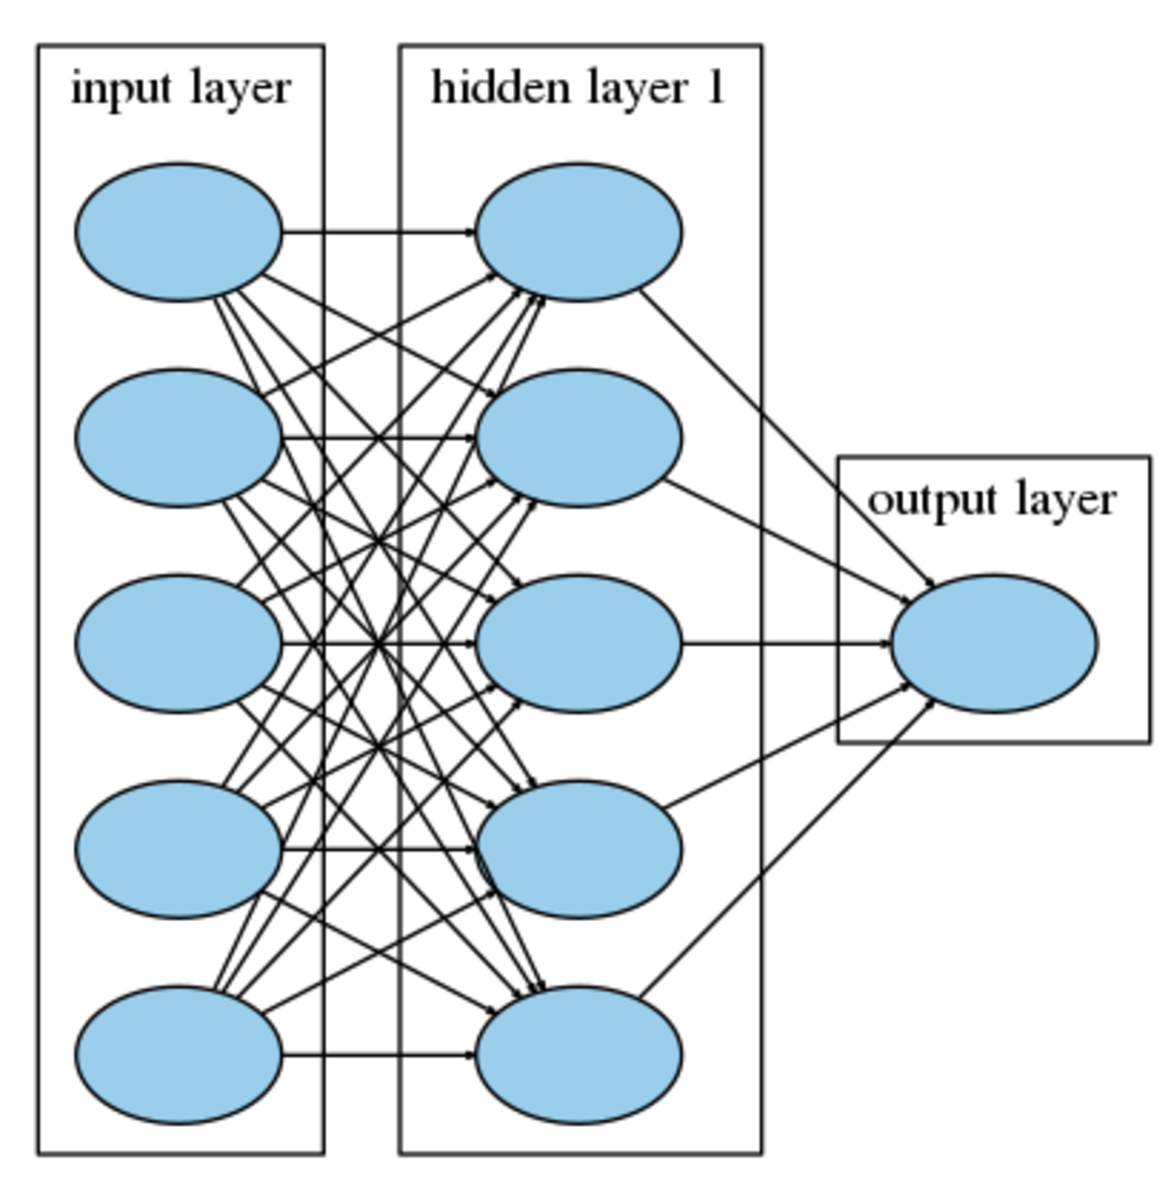
\includegraphics[height=0.3\textwidth]{ann_2_visualization.png}};
      \end{tikzpicture}
    \end{center}
\end{frame}

\begin{frame}
    \frametitle{History (stay with me it's fun!)}
    \begin{center}
      \begin{itemize}
        \item Field revolutionized in the 2000s by deep learning
        \item Advances it algorithms $\rightarrow$ training with many layer is possible
        \item More statistics (big data)
        \item Massive boost in computing power (due to GPUs)
      \end{itemize}


      \vspace{1em}
      \textbf{Deep neural network}


      \begin{tikzpicture}
        \node[anchor=south west,inner sep=0] (image) at (0,0) {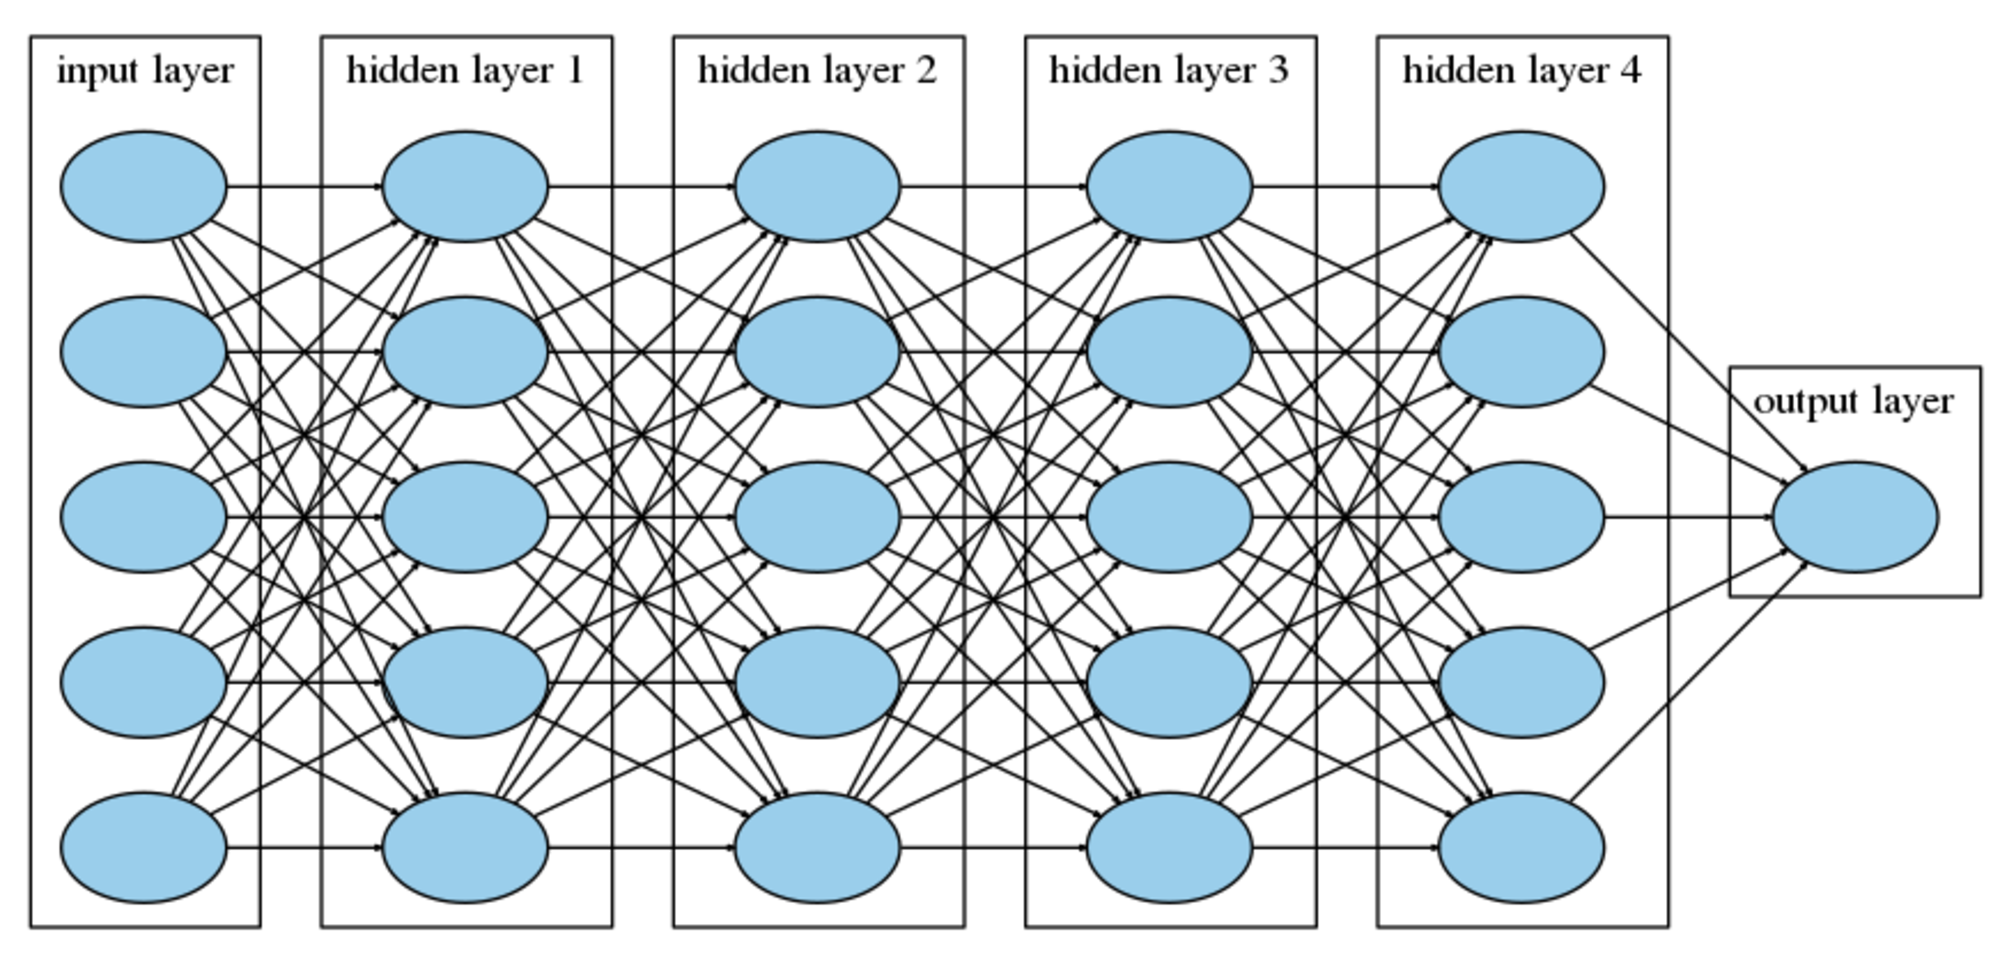
\includegraphics[height=0.3\textwidth]{ann_3_visualization.png}};
      \end{tikzpicture}
    \end{center}
\end{frame}

\begin{frame}
  \frametitle{Today (all aboard the hype train)}
    \begin{center}
      \begin{columns}
	    \column{0.65\textwidth}
      \begin{itemize}
        \item Representation learning
        \item Feed in low-level features \\ $\rightarrow$ learn high-level features automatically
        \item HEP is getting into it as well!
      \end{itemize}
	    \column{0.35\textwidth}
      \begin{tikzpicture}
        \node[anchor=south west,inner sep=0] (image) at (0,0) {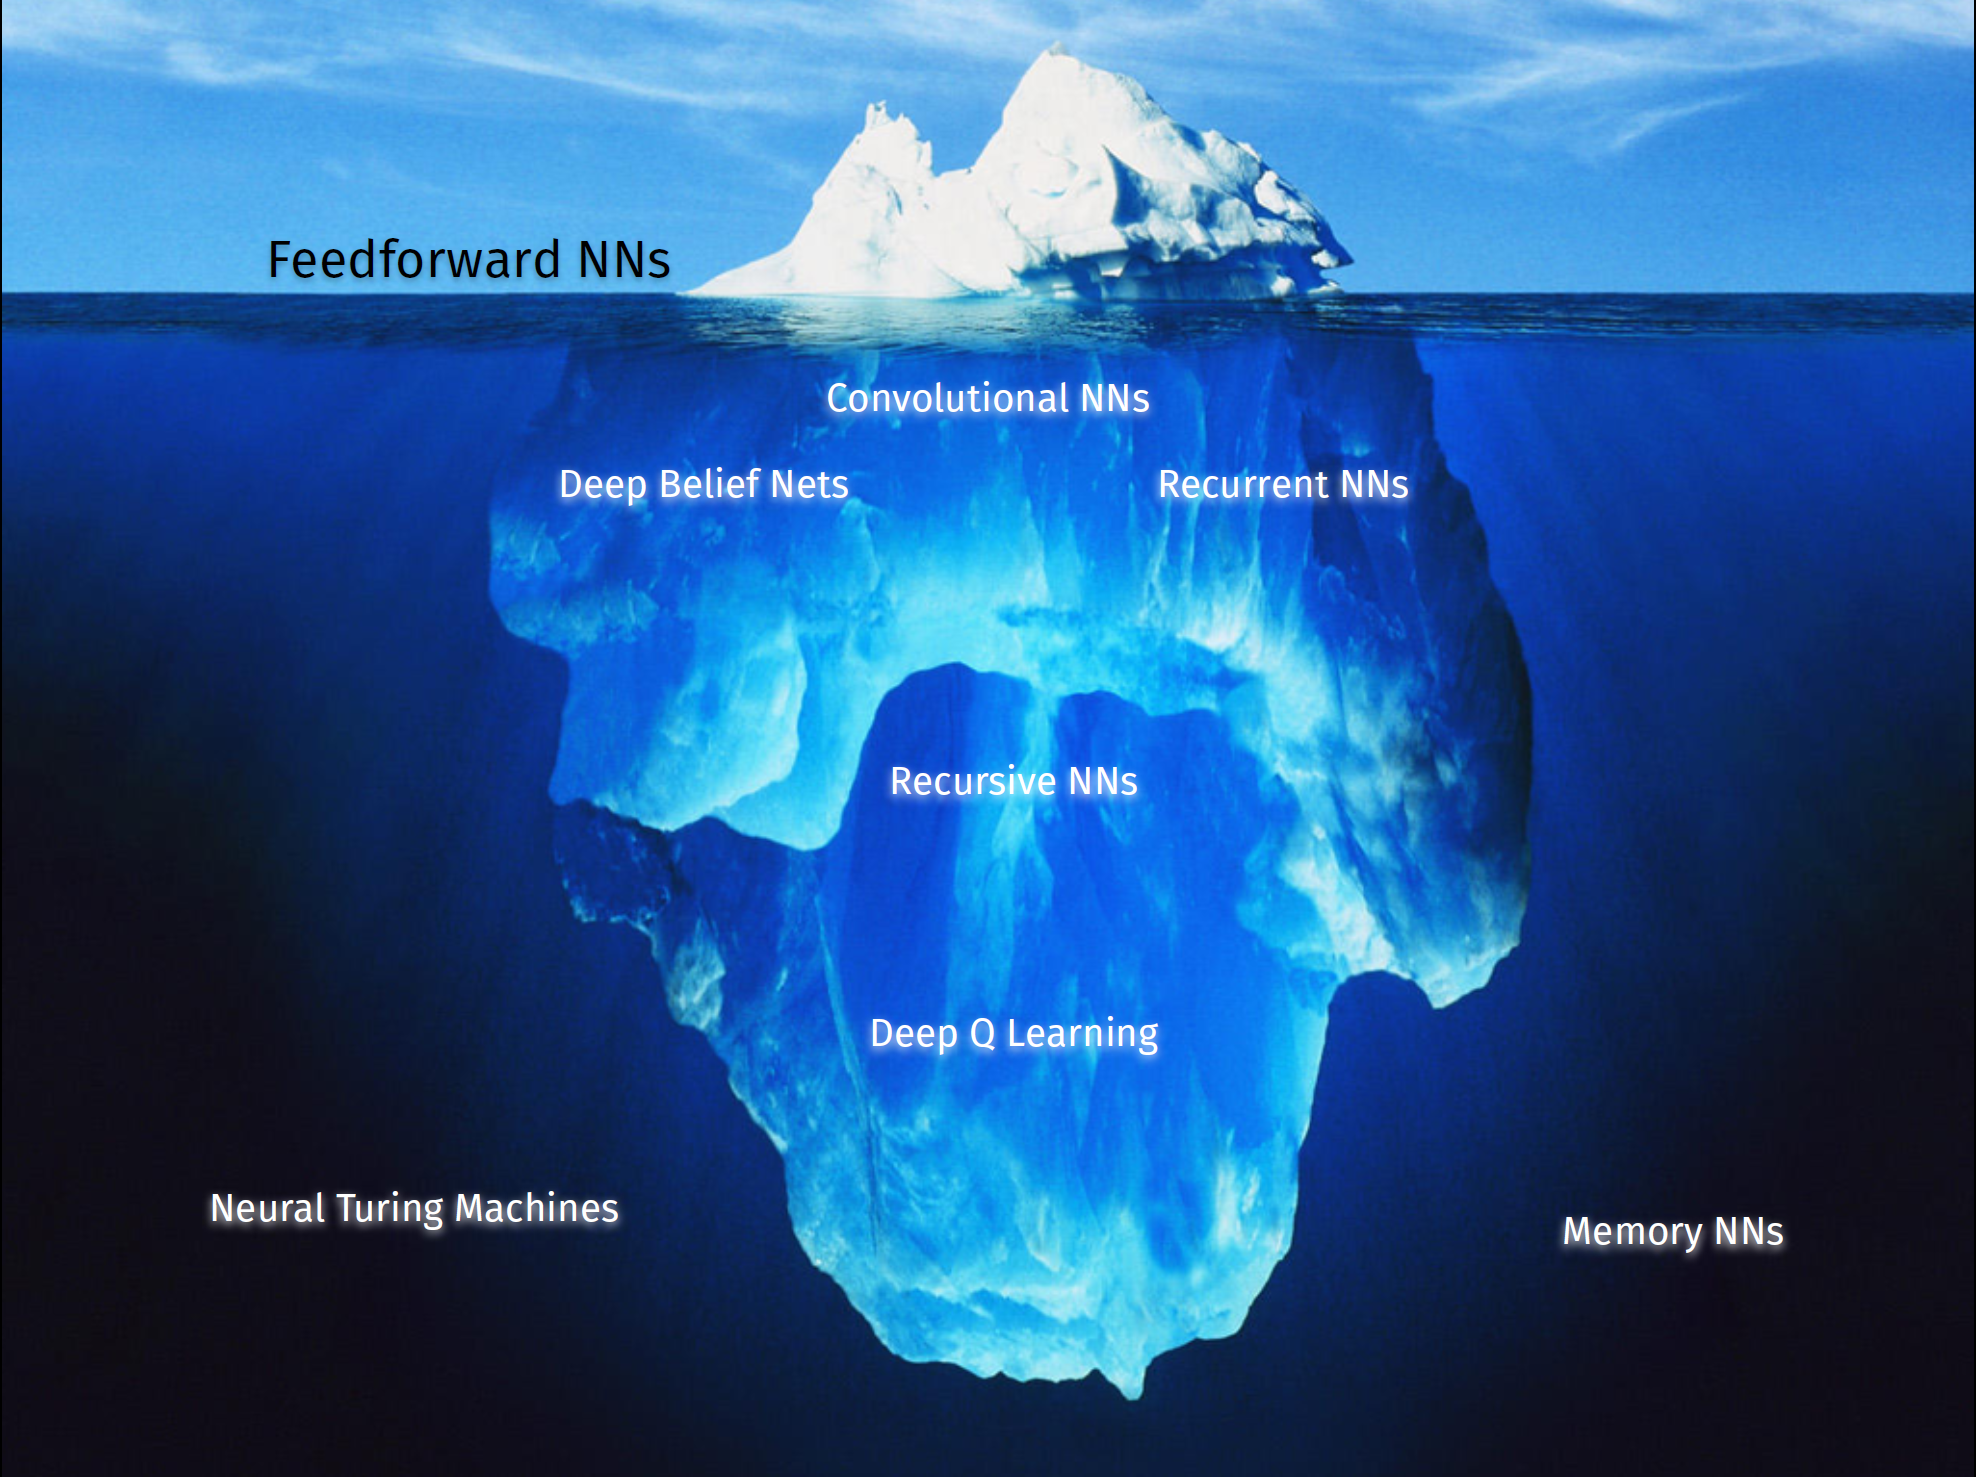
\includegraphics[width=\textwidth]{ice.png}};
      \end{tikzpicture}
      \end{columns}


      \vspace{0.5em}
      \textbf{Deep neural network}


      \begin{tikzpicture}
        \node[anchor=south west,inner sep=0] (image) at (0,0) {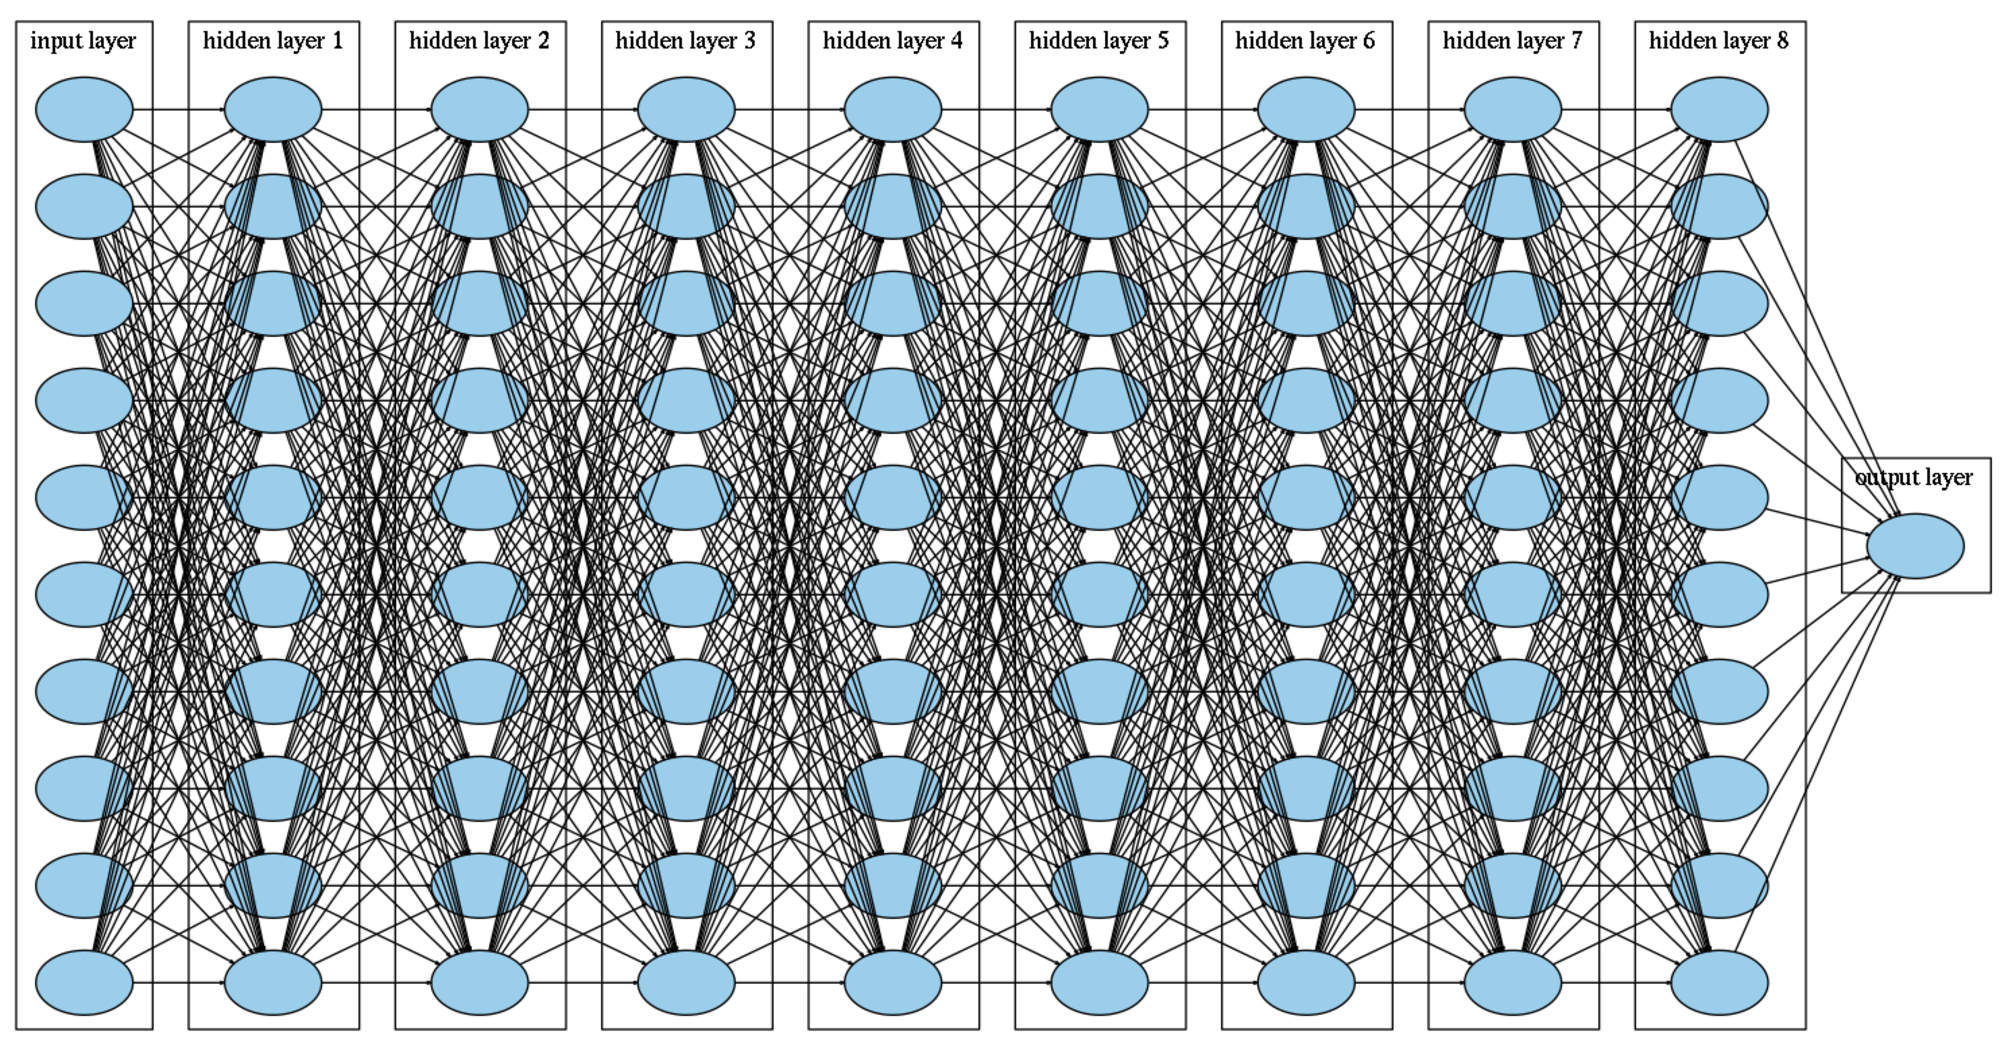
\includegraphics[height=0.3\textwidth]{deep_visualization.png}};
      \end{tikzpicture}

    \end{center}
\end{frame}

\begin{frame}
  \frametitle{Physics example}
    \begin{center}
      \vspace{-1em}
      \begin{tikzpicture}
        \node[anchor=south west,inner sep=0] at (0,0) {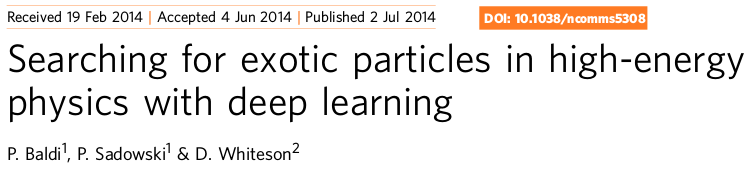
\includegraphics[width=\textwidth]{DLHEP.png}};
        \node[anchor=south west,inner sep=0] at (0,-5) {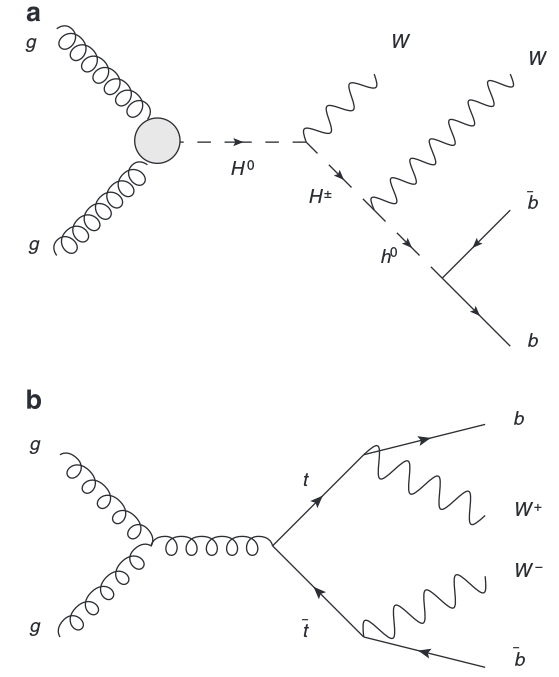
\includegraphics[width=0.4\textwidth]{DLHEP_process.png}};
        \node[anchor=south west,inner sep=0] at (5,-3) {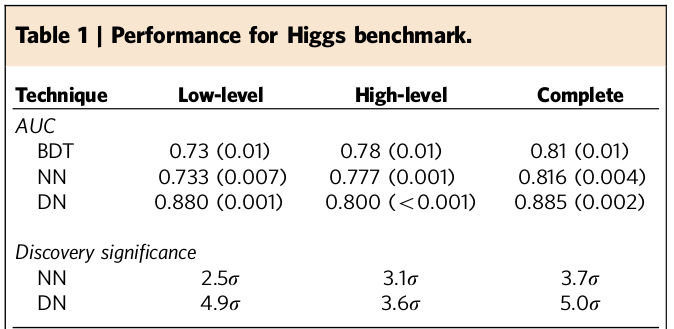
\includegraphics[width=0.6\textwidth]{DLHEP_result.png}};
      \end{tikzpicture}
    \end{center}
\end{frame}

